\newpage
\section*{Problem 3:}
\begin{enumerate}
\item In order to generalize the fast elliptical solver, we need account for the nonzero boundary conditions and add it to the $F$ matrix. Let $V_{jk} \approx V(x_{i}, y_{k}) \in \mathbb{R}^{m\times m}$ and $f_{j,k} \approx f(x_{j}, y_{k}) \in \mathbb{R}^{m\times m}$ where $m$ is the number of grid point in each dimension and $i,k = 1, \dots, m$. The centered finite-difference formula is 
$$
4 v_{jk} - v_{j-1,k} - v_{j+1,k} - v_{j, k-1} - v_{j,k+1} = h^{2}f_{j,k}, \quad j,k=1, \dots, m
$$
The compact formulation of the 2D centered finite-difference from which we derived the FFT-based fast elliptical solver is 

$$
T_{m}V + VT_{m} = h^{2}F
$$

where $h=\frac{1}{m+1}$ and $T_{m}\in \mathbb{R}^{m\times m}$ is the centered finite-difference in 1D i.e., 

$$
T_{m} = 
\setcounter{MaxMatrixCols}{11}
\begin{bmatrix}
2 & -1& 0 & \cdots & 0\\
-1& 2 & -1& \cdots  & \vdots\\
\vdots & \ddots & \ddots & \ddots & \vdots\\
\vdots &   & \ddots & \ddots & -1\\
0 & \cdots & 0 & -1 & 2\\
\end{bmatrix}
$$
The nonzero boundary conditions only changes $F$  when $j=1 \text{\ or\ } m$ and $k=1 \text{\ or\ } m$ as follows. With zero boundary condition at $j=1$, $v_{j-1,k} = v_{0,k}$ ($k=1, \dots m $) used to not affect $F$ but now since $v_{0,k} = c0(y)$, we need to add this to the RHS $F$. We do the same thing for the remaining three boundaries. This will adjust $F$ such that 
$$F(1,:) = F(1,:) + \frac{b_{0}(x)}{h^{2}}$$
$$F(m,:) = F(m,:) + \frac{b_{1}(x)}{h^{2}}$$
$$F(:,1) = F(:,1) + \frac{c_{0}(y)}{h^{2}}$$
$$F(:,m) = F(:,m) + \frac{c_{1}(y)}{h^{2}}$$

Note that we divide by $h^{2}$ since $F$ will be multiplied by $h^{2}$ and so it cancels out. We substitute the discrete values $x$ and $y$ at grid point $j$ in $b_{0}(x), b_{1}(x), c_{0}(y),\text{\ and \ } c_{1}(x)$ as $x= \frac{j}{m+1}$ and $y= \frac{j}{m+1}$. After adjusting $F$, the same derivation will follow as given in the class. 

\item Function \texttt{FFTSolver()} implements the FFT-based solver. 

\item To determine function $b_{0}$, $b_{1}$, $c_{0}$, and $c_{1}$ we simply plug in their definition in  $v(x,y)$ definition

\begin{align*}
& b_{0} = v(x,0) = 0 \\
& b_{1} = v(x,1) = x^{\alpha} cos(\beta \pi x) sin(\gamma \pi) \\
& c_{0} = v(0,y) = 0^{\alpha}sin(\gamma \pi y)\\
& c_{1} = v(1,y) = cos(\beta \pi)sin(\gamma \pi y) 
\end{align*}

$f$ can be determined from its definition i.e., $f(x,y) = -\frac{\partial^{2} v(x,y)}{\partial x^{2}} - \frac{\partial^{2} v(x,y)}{\partial y^{2}}$ where
\begin{align*}
& \frac{\partial^{2} v(x,y)}{\partial x^{2}} = sin(\gamma \pi y) \left[ 
\left( \alpha(\alpha-1)x^{\alpha-2} + \beta^{2} \pi^{2} x^{\alpha}\right)cos(\beta \pi x) - 2\alpha \beta \pi x^{\alpha -1} sin(\beta \pi x) \right]\\
& \frac{\partial^{2} v(x,y)}{\partial y^{2}} = -\alpha^{2}\pi^{2} x^{\alpha} cos(\beta \pi x)sin (\gamma \pi y)
\end{align*}

\item Figure~\ref{p4} shows the chosen $m$ for different test cases and the corresponding absolute error. We choose the grid size such that error is always less than 0.0001. \Cref{fig:case1,fig:case2,fig:case3,fig:case4,fig:case5} show the right-hand side function $f$, the exact solution $v$, and the computed solution for all the test cases. 

\begin{figure}[tbh]
 \centering    
\begin{tabular}{ |p{5cm}|| p{1cm}|p{1.5cm}|}
 \hline
 Test Case &  $m$  & Error \\ \hhline{|=|=|=|}
 \hline
 (\rom{1}) $\alpha = 0, \beta =1, \gamma = 1$ & 60  & 0.000075\\
 (\rom{2}) $\alpha = 1, \beta =2, \gamma = 1$ & 200  & 0.000069\\
 (\rom{3}) $\alpha = 2, \beta =2, \gamma = 3$ & 150  & 0.000078\\
 (\rom{4}) $\alpha = 5, \beta =2, \gamma = 3$ & 80  & 0.000048\\
 (\rom{5}) $\alpha = 5, \beta =3, \gamma = 5$ & 200  & 0.000094\\
 \hline
\end{tabular} 
\caption{Chosen $m$ and absolute error for different test cases}
\label{p4}
\end{figure} 


\begin{figure}
\centering        
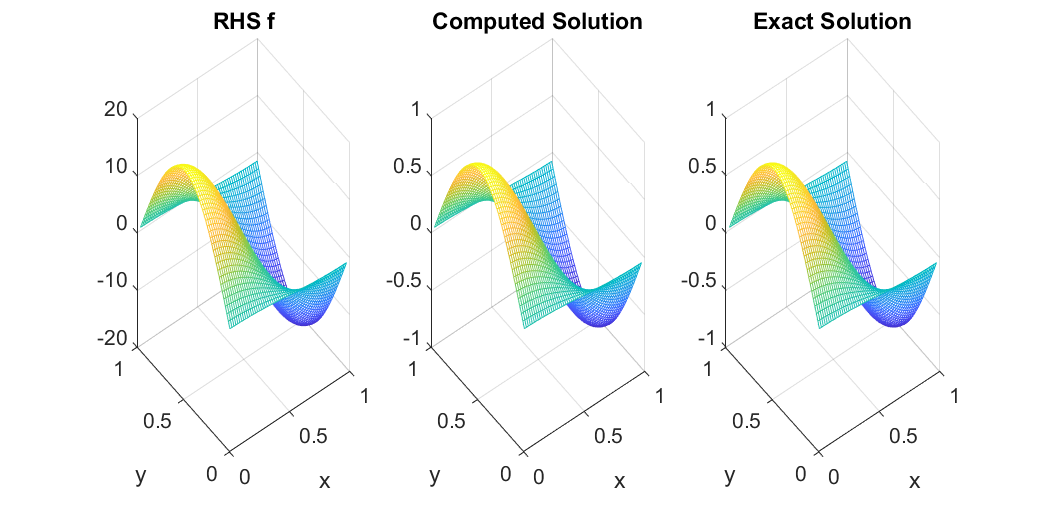
\includegraphics[width=1.0\textwidth]{../code/Case_i.png}
   \caption{Test Case \rom{1}}
   \label{fig:case1}
\end{figure}


\begin{figure}
\centering        
 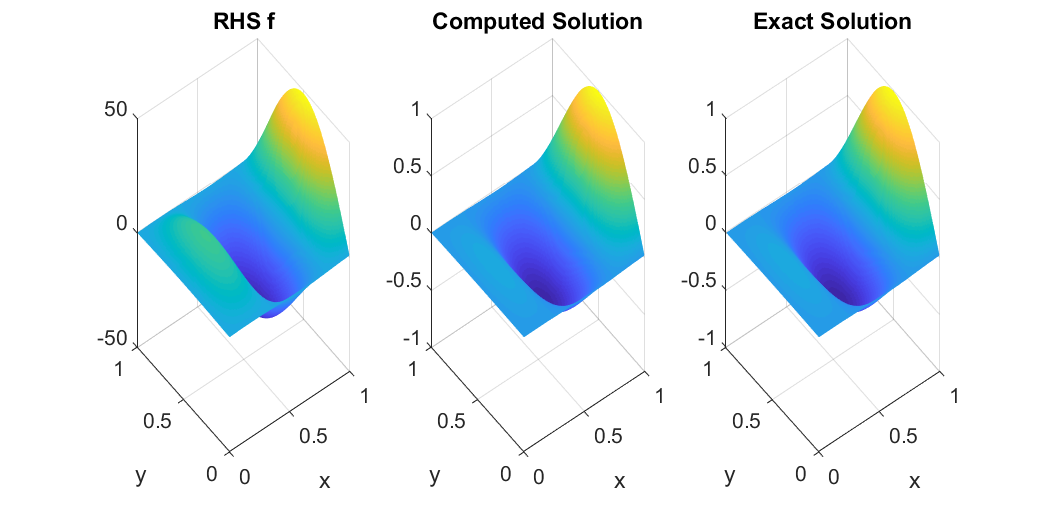
\includegraphics[width=1.0\textwidth]{../code/Case_ii.png}
   \caption{Test Case \rom{2}}
   \label{fig:case2}
\end{figure}

\begin{figure}
\centering        
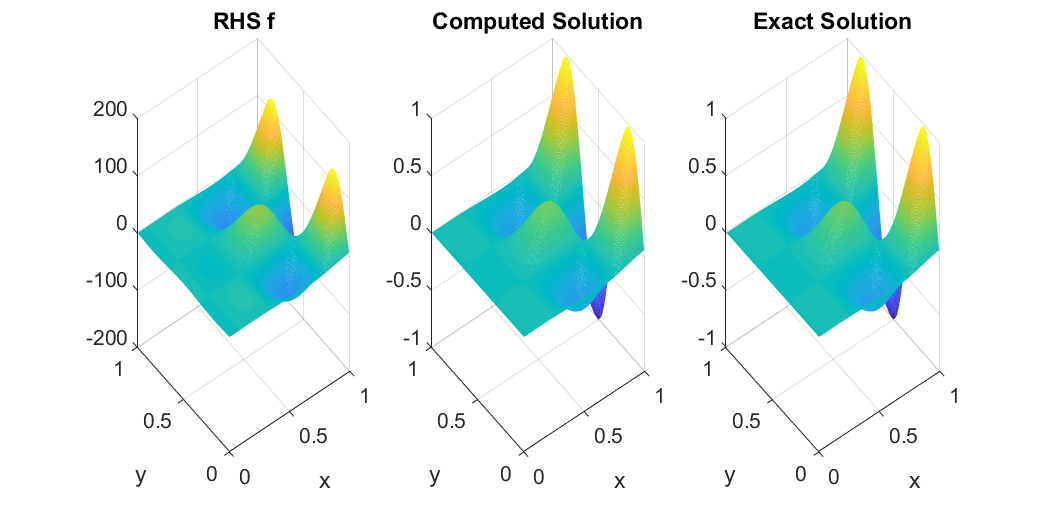
\includegraphics[width=1.0\textwidth]{../code/Case_iii.png}
   \caption{Test Case \rom{3}}
   \label{fig:case3}
\end{figure}

\begin{figure}
\centering        
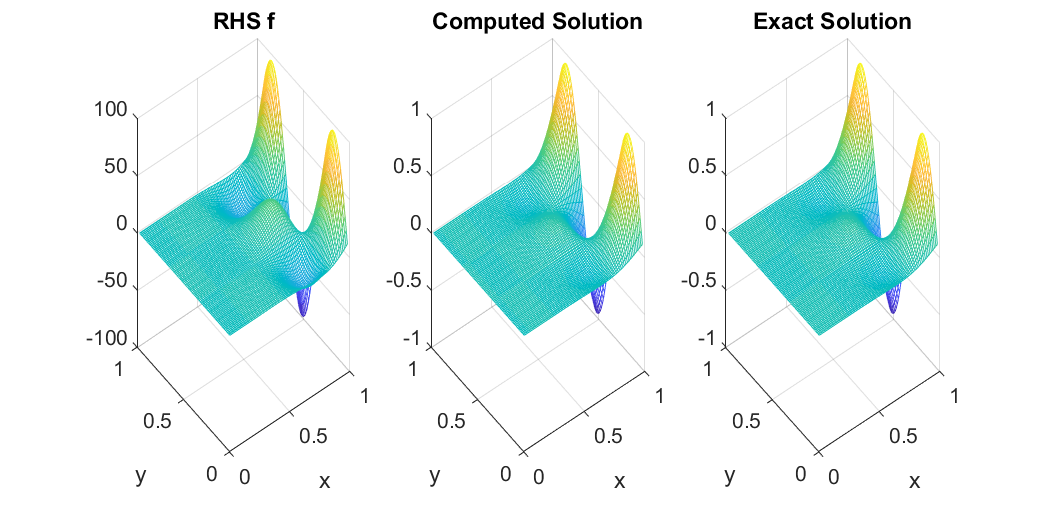
\includegraphics[width=1.0\textwidth]{../code/Case_iv.png}
   \caption{Test Case \rom{4}}
   \label{fig:case4}
\end{figure}

\begin{figure}
\centering        
 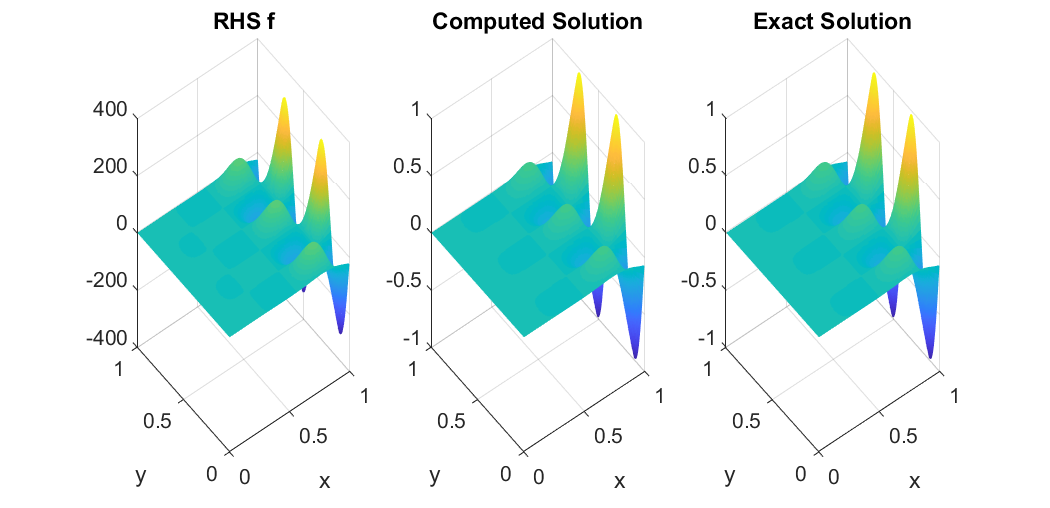
\includegraphics[width=1.0\textwidth]{../code/Case_v.png}
   \caption{Test Case \rom{5}}
   \label{fig:case5}
\end{figure}


\end{enumerate}